\classheader{09-06-2017}

\section*{The Pullback Topology}

Let $(X,\mathcal{A})$ be a topological space and $Y$ some set.  Given a map $f:X\rightarrow Y$, $Y$ inherits a topology from $X$ where $V\subset Y$ is open if and only if $f^{-1}(V)\subset X$ is open.

\definition{This topology on $Y$ is called the \textbf{pullback topology}.}

The pullback topology is the finest topology on $Y$ which makes $f$ a continuous map.

\example{Take $f:(-1,1)\rightarrow \mathbb{R}$ with $f(x)=x$ and the standard topology on each.  The pullback topology on $\mathbb{R}$ has open sets $\emptyset$ and $\mathbb{R}$, whose inverse images are themselves.  Also, any set in $\mathbb{R}$ which does not intersect the open interval $(-1,1)$, as all of these sets have empty inverse image.  Finally, any set which is open in $(-1,1)$ or whose intersection with $(-1,1)$ is open is also open in the pullback topology.}

\section*{Group Actions and Fundamental Regions}

Let’s think about $\mathbb{Z}^2$ as a group action on $\mathbb{R}^2$ , where applying $(a, b) \in \mathbb{Z}^2$ to $(x, y) \in \mathbb{R}^2$ means
shifting $(x, y)$ right by $a$ and up by $b$ (left, down if $a$ or $b$ is negative, of course). We write this
as $\mathbb{Z}^2$ acts on $\mathbb{R}^2$ by $(a, b) . (x, y) = (x + a, y + b)$. This establishes an equivalence relation on $\mathbb{R}^2$ :
$(x_0 , y_0 ) ∼ (x_1 , y_1 )$ if there exists $(a, b) \in \mathbb{Z}^2$ such that $(a, b). (x_0 , y_0 ) = (x_1 , y_1 )$.
This divides $\mathbb{R}^2$ into $1 \times 1$ squares, where each square is equivalent to any other, and we identify
the left and right edges and the top and bottom edges, but no two points in the interior of any
given square are equivalent. We call the squares fundamental regions.

\definition{A \textbf{fundamental region} of a group action and is the (closure of) largest region such
	that no two interior points are identified with respect to the induced equivalence relation.}

\example{The fundamental region described above, the square with opposite edges identified,
	defines a torus.}


\begin{figure}[!htb]
	\centering
	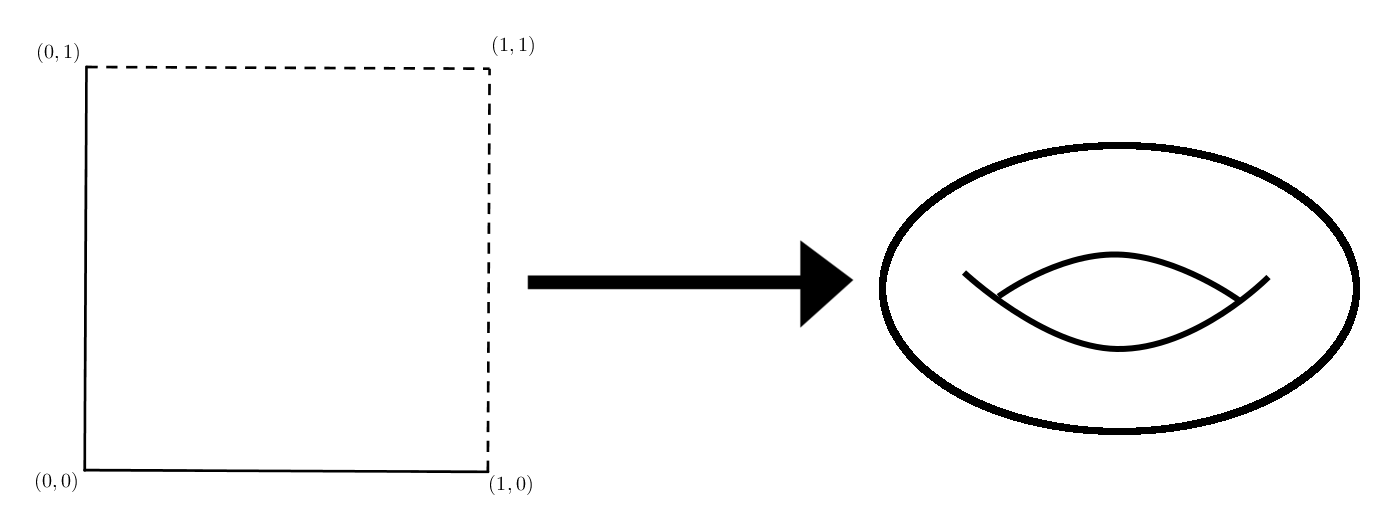
\includegraphics[width=0.7\linewidth]{images/frtorus}
	\caption{}
	\label{fig:frtorus}
\end{figure}

	

	
	

Open sets in the torus $\mathbb{R}$ are $\emptyset$ and $\mathbb{T}$, and the intersection of any standard open set with the fundamental region.  This is the same as the inherited subspace topology from $\mathbb{R}^2$.

\example{If we consider $\mathbb{R}^2/\mathbb{Z}$, where $a\in \mathbb{Z}$ acts on $\mathbb{R}^2$ by $a.(x,y)=(x+a,y)$.  A fundamental domain of this action is a vertical strip of unit width.  Again this inherits a subspace topology from $\mathbb{R}^2$.}



	







	\begin{figure}[!htb]
		\centering
		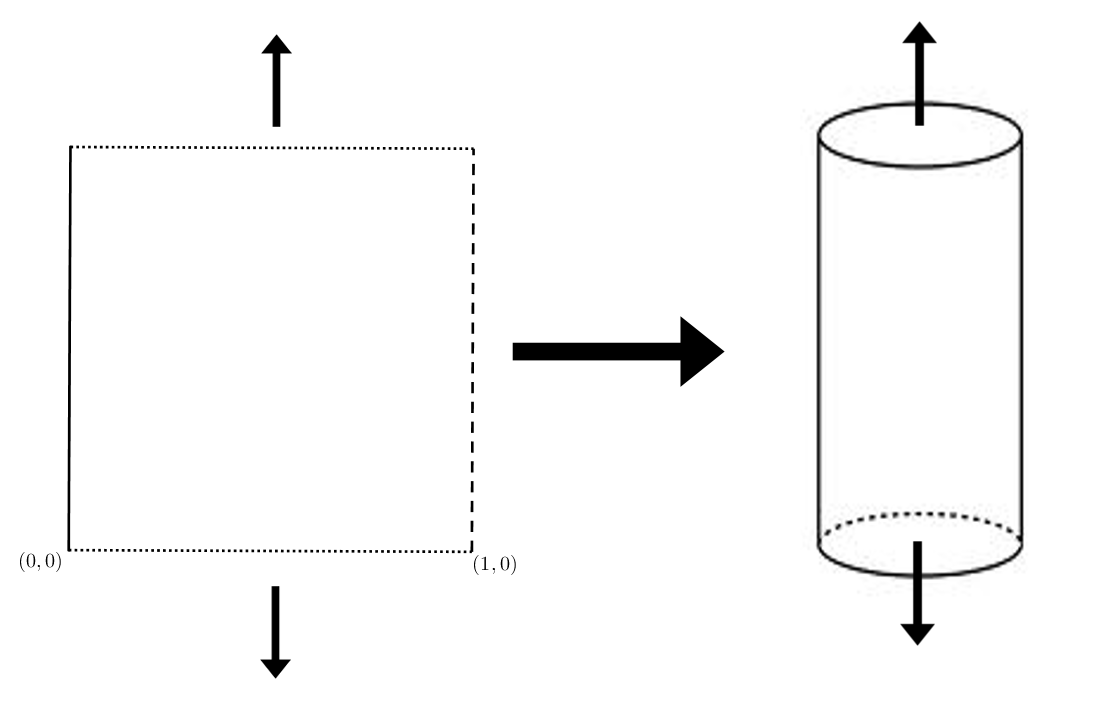
\includegraphics[width=0.7\linewidth]{images/frcyl}
		\caption{}
		\label{fig:frcyl}
	\end{figure}
	
	
	
	
	
\example{Consider again $\mathbb{R}^2/\mathbb{Z}$ but this time with the group action $a.(x,y)=(x+a,(-1)^ay)$.  The fundamental region is still a strip of unit width, but this time instead of identifying points on
	the boundary with their horizontal translation, we identify them with their horizontal translation
	composed with reflection about the $x$-axis. This space is homeomorphic to an infinite Moebius strip,
	which is difficult to draw.}


\example{Consider the equivalence relation on $\mathbb{R}^2$ described by $(x,y)\sim (x,y)$, $(0,y)\sim(1,y)$, and $(x,0)\sim(1-x,1)$.  The fundamental region again is a square with the left and right edges identified
	by simple translation, but the top and bottom edges are now identified by translation plus a flip
	across the square’s vertical axis of symmetry. This is homeomorphic to the Klein bottle, which is,
	again, hard to draw.}

\example{The previous example where we also identify the left and right edges by translation and
	a flip is called the real projective plane, denoted $\mathbb{R}P^2$
	. Both vertical and horizontal strips of this
	space look like Moebius strips. This is, once again, not easy to draw.}

\example{This one we can draw! Take the unit square as the fundamental region, but identify
	the top and left edge with each other by symmetry about the corner where they intersect, and do
	the same for the bottom and right edge. This space is homeomporhic to the 2-sphere $\mathbb{S}^2$
	.}
	
	
\begin{figure}[!htb]
\centering
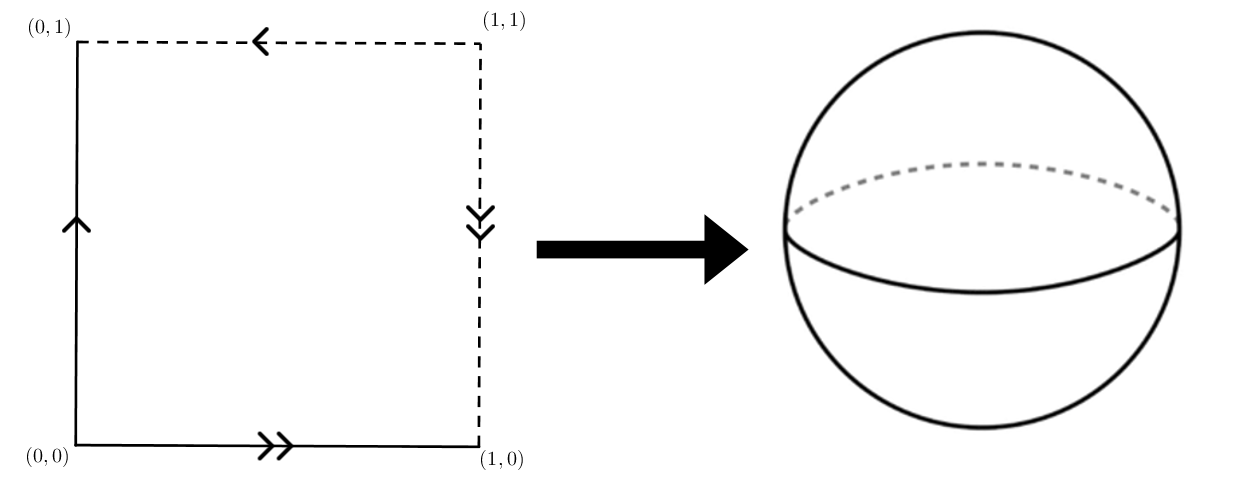
\includegraphics[width=0.7\linewidth]{images/frs2}
\caption{}
\label{fig:frs2}
\end{figure}
	
	
	
	

